\documentclass[]{beamer}

\usepackage[utf8]{inputenc}
\usepackage[danish]{babel}
\usepackage[T1]{fontenc}
\usepackage{graphicx}
\usepackage{amsmath}
\usepackage{hyperref}
\usepackage{enumerate}
\usepackage{url}

\renewcommand{\emptyset}{\varnothing}
\newcommand{\ignore}[1]{}
\newcommand{\f}[1]{\textcolor{red}{#1}}

%\let\originaltextperiodcentered\textperiodcentered
\renewcommand{\textperiodcentered}{\ensuremath{\cdot}}
\newcommand{\explain}[2]{\underset{\mathclap{#2}}{\underbrace{#1}}}
\newcommand{\putat}[3]{\begin{picture}(0,0)(0,0)\put(#1,#2){#3}\end{picture}}

\def\imagetop#1{\vtop{\null\hbox{#1}}}

\newenvironment<>{varblock}[2][\textwidth]{%
  \setlength{\textwidth}{#1}
  \begin{actionenv}#3%
    \def\insertblocktitle{#2}%
    \par%
    \usebeamertemplate{block begin}}
  {\par%
    \usebeamertemplate{block end}%
  \end{actionenv}}

\setbeamertemplate{navigation symbols}{} 
\setbeamertemplate{items}[circle]
\useoutertheme{infolines} 
\setbeamercovered{transparent=40} 

\title{3. Seminar EVU RegAut}
\author{Sigurd Meldgaard}
\date{1. oktober 2010}

\AtBeginSection[]
{
   \begin{frame}
       \frametitle{Plan}
       \tableofcontents[currentsection]
   \end{frame}
}

\begin{document}
\maketitle
\section{Lukketheds- og afgorlighedsegenskaber}

\begin{frame}
  \frametitle{Lukketheds og afgørlighedsegenskaber}
  \begin{itemize}
  \item Lukkethed under $\cup, \cap, ', \cdot, {}^*$ 
  \item Lukkethed under homomorfi og invers 
    homomorfi 
  \item ``Pumping''-lemmaet 
  \item Beslutningsproblemer: membership,  
    emptiness,finiteness subset, equality 
  \item Beslutningsprocedurer i Java-pakken
  \end{itemize}
\end{frame}

\begin{frame}
\frametitle{Lukkethedsegenskaber}
Givet to regulære sprog $L_1, L_2$
\begin{itemize}[<+->]
\item er $L_1 \cap L_2$ regulært
\item er $L_1 \cup L_2$ regulært
\item er $L_1'$ regulært
\item er $L_1L_2$ regulært
\item er $L_1^*$ regulært
\end{itemize}
Ja, det beviste vi første seminar (produktkonstruktionen)
\end{frame}

\begin{frame}
\frametitle{Kontraponering, (Contraposition)}
\begin{itemize}[<+->]
\item Lukkethedsegenskaber kan vise at sprog \emph{ikke} er regulære.
\item Fx: Klassen af regulære sprog er lukket under $\cap$
\item Antag vi har bevist, at sproget S ikke er  
regulært 
\item Hvis $S = P \cap R$ og $R$ er regulært, så kan  
$P$ ikke være regulært.
\end{itemize}
\end{frame}

\begin{frame}
\frametitle{Homomorfier}
\begin{itemize}[<+->]
\item Antag $g: \Sigma_1 \rightarrow \Sigma_2^*$ hvor $\Sigma_1$ og
  $\Sigma_2$ er alfabeter
\item  Definer  $h: \Sigma_1^* \rightarrow \Sigma_2^*$ ved 
   \[
   h(x) = \begin{cases}\Lambda &\text{ hvis }x=\Lambda \\
     h(y)g(a)  & \text{ hvis }x=ya, y\in\Sigma_1^*, a\in\Sigma_1
\end{cases}
   \]
\item  h opfylder at h(xy)=h(x)h(y) og kaldes en  
homomorfi 
\item  Definer  $h(L) = \{ h(x) | x\in L \}$  for alle $L\subseteq\Sigma_1^*$
\item  og $h-1(L) = \{ x | h(x)\in L \}$  for alle $L\subseteq\Sigma_2^*$ 
\item Se opg. [Martin, opg.4.46] p. 166.
\end{itemize}
\end{frame}

\begin{frame}
\frametitle{Regularitet og homomorphier}
\begin{itemize}[<+->]
\item Hvis $h: \Sigma_1^* \rightarrow \Sigma_2^*$ er en homomorphi og
  $L\subseteq \Sigma_1^*$ er et regulært sprog, så er $h(L)$ også regulært.
\item Hvis $h: \Sigma_1^* \rightarrow \Sigma_2^*$ er en homomorphi og
  $L\subseteq \Sigma_2^*$ er et regulært sprog, så er $h^{-1}(L)$ også regulært.
\end{itemize}
Dvs. klassen af regulære sprog er lukket både under homomorfi og
invers homomorfi.
\end{frame}

\begin{frame}
\frametitle{Eksempel}
\begin{itemize}[<+->]
\item Er følgende sprog over alfabetet $\Sigma=\{0,1,2\}$ regulært?  
   $L = \{ x2y | y=reverse(x), x,y\in\{0,1\}^* \}$ 
\item  Vi ved (fra første seminar) at sproget  
   $pal = \{ x\in\{0,1\}^* | x=reverse(x) \}$  
ikke er regulært 
\item  En (utilstrækkelig) intuition: 
$L$ minder om $pal$, men måske symbolet $2$, der markerer  
midten af strengen, gør, at vi kan lave en FA for $L$?
\end{itemize}
\end{frame}

\begin{frame}
\frametitle{Eksempel, fortsat}
\begin{itemize}[<+->]
\item  Definer tre funktioner  $g1,g2,g3:  \{0,1,2\}\rightarrow\{0,1\}^*$  ved 
\[g_1(0)=0,\ g_2(0)=0,\ g_3(0)=0 \]
\[g_1(1)=1,\ g_2(1)=1,\ g_3(1)=1 \]
\[g_1(2)=\alert{\Lambda},\ g_2(2)=\alert{0},\ g_3(2)=\alert{1} \]
\item  Og lad $h1,h2,h3$ være de tilhørende homomorfier 
\item  $h1(L) \cup h2(L) \cup h3(L) = pal$ 
\item  Så L er \emph{ikke} regulært, idet pal ikke er regulært og klassen  
af regulære sprog er lukket under forening og homomorfi
\end{itemize}
\end{frame}

\begin{frame}
\frametitle{Bevis, del 1 (Øvelse)}
\begin{itemize}[<+->]
\item Hvis h: $\Sigma_1^*\rightarrow\Sigma_2^*$ er en homomorfi og
  $L\subseteq\Sigma_1^*$ er et regulært sprog, så er $h(L)$ også regulært
  \item Bevis: Strukturel induktion i regulære udtryk...
    (erstat hver $a\in\Sigma_1$ i udtrykket med $h(a)$).
\end{itemize}
\end{frame}

\begin{frame}
\frametitle{Bevis, del 2}
\begin{itemize}[<+->]
\item Hvis h: $\Sigma_1^*\rightarrow\Sigma_2^*$ er en homomorfi og
  $L\subseteq\Sigma_2^*$ er et regulært sprog, så er $h^{-1}(L)$ også regulært
  \item Bevis: givet en FA $M=(Q, \Sigma_2, q_0, A, \delta)$ så $L(M)=L$.
    Definer en ny FA $M' = (Q, \Sigma_1, q_0, A, \delta ')$ hvor
    $\delta'(q,a) = \delta^*(q,h(a))$
  \item Bevis nu at $L(M')=h^{-1}(L)=h^{-1}(L(M))$.
  \item Brug induktion i en
    streng $x\in L(M)$ og vis at $\delta'^*(q_0,x) =
    \delta^*(q_0,h(x))$.
\end{itemize}
\end{frame}

\section{Pumping lemmaet}

\begin{frame}
\frametitle{Endnu en egenskab ved regulære sprog}
\begin{itemize}[<+->]
\item Antag $M=(Q, \Sigma, q_0, A, \delta)$ er en FA og $\exists x\in L(M): |x| \geq |Q|$
\item Ved en kørsel af $x$ på $M$ vil mindst én af tilstandene blive
  besøgt mere end en gang.
    \begin{center}
    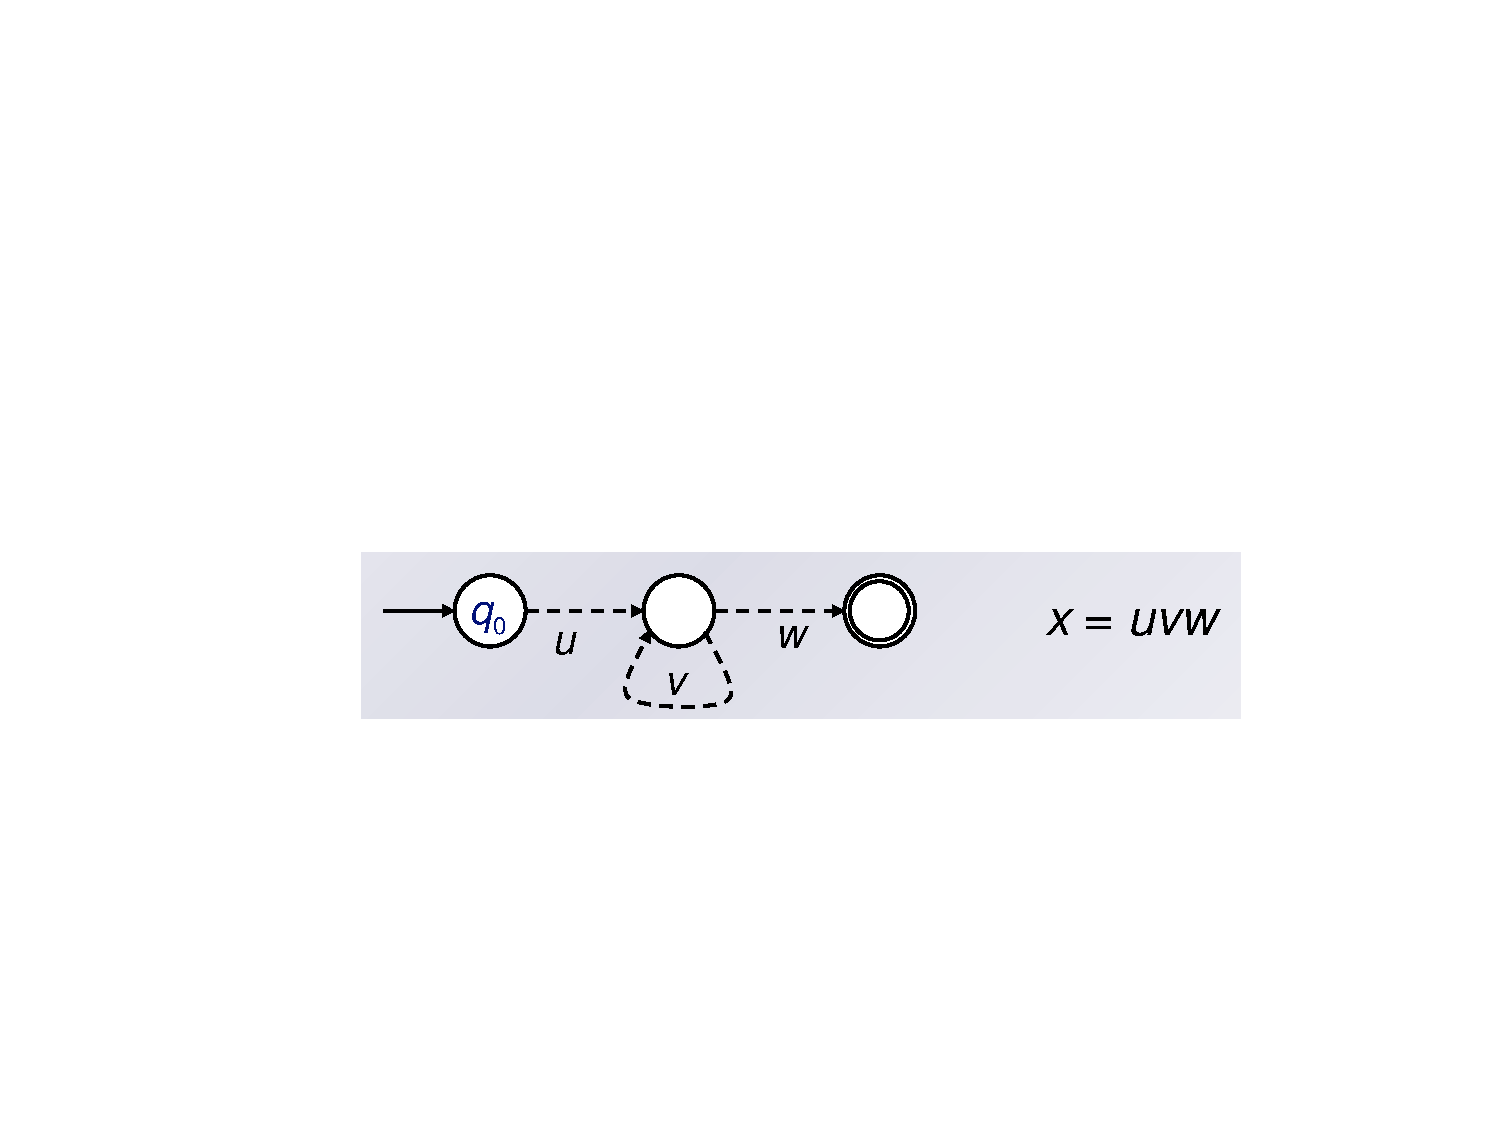
\includegraphics[scale=.40]{images/pumping}
    \end{center}
\item Se på den første af disse tilstande, nu kan vi se at:
  $\exists u,v,w\in \Sigma^*: x=uvw \wedge |uv| \leq |Q| \wedge |v|>0 \wedge
  \delta^*(q_0,u)=\delta^*(q_0,uv)$
\end{itemize}
\end{frame}

\begin{frame}
\frametitle{``Pumping''-lemmaet for regulære sprog}
Hvis $L$ er et regulært sprog så gælder:

\hspace{1cm}$\exists n>0:$\\
\pause
\hspace{2cm}$\forall x\in L \text{ hvor } |x| \geq n:$\\
\pause
\hspace{3cm}$\exists u,v,w\in \Sigma^*:$\\
\pause
\hspace{4cm}$(x = uvw) \pause \wedge (|uv|\leq n) \pause \wedge (|v| > 0) \wedge$\\
\pause
\hspace{4cm}$(\forall m\geq 0: uv^mw\in L)$\\
\pause
\end{frame}

\begin{frame}
\frametitle{``Pumping''-lemmaet for \alert{ikke}-regulære sprog}
Dette resultat kan kontraponeres:
\pause
\setbeamercolor{lowercol}{fg=black,bg=green}% 
\begin{beamerboxesrounded}[lower=lowercol,shadow=true]{}
  Hvis det gælder om $L$\\
\pause
\hspace{1cm}$\forall n>0:$\\
\pause
\hspace{2cm}$\exists x\in L \text{ hvor } |x| \geq n:$\\
\pause
\hspace{3cm}$\forall u,v,w\in \Sigma^*:$\\
\pause
\hspace{4cm}$(x = uvw) \wedge (|uv|\leq n) \wedge (|v| > 0) \wedge$\\
\pause
\hspace{4cm}$(\exists m\geq 0: uv^mw\not\in L)$\\
\pause
Så kan $L$ ikke være regulært.
\end{beamerboxesrounded}
\end{frame}
\xdefinecolor{dg}{rgb}{0.2,.6,.2}
\xdefinecolor{dr}{rgb}{0.6,.2,.2}

\begin{frame}
\frametitle{Pumping-lemmaet som ``kvantor-spil''}
\begin{itemize}[<+->]
\item  Antag vi prøver at vise, at L er ikke-regulært 
\item  Vi skal vise noget på form 
 $\forall n\ldots:   \exists x\ldots:  \forall u,v,w \ldots:  \exists m\ldots:  \ldots$ 
\item  ``Fjenden'' vil prøve at modarbejde os
  \begin{enumerate}
  \item Fjenden vælger {\color{dr}$n$}
  \item Vi vælger {\color{dg}$x$}   (efter reglerne, dvs. så $x\in L$ og $|x|\geq n$) 
  \item Fjenden vælger {\color{dr}$u,v,w$}   (efter reglerne\ldots) 
  \item Vi vælger \color{dg}{$m$}
  \end{enumerate}
\item
Hvis vi uanset fjendens valg kan opnå at $uv^mw\not\in L$, 
så har vi vundet, dvs. bevist at $L$ er ikke-regulært.
\end{itemize}
\end{frame}

\begin{frame}
\frametitle{Eksempel 1}
Lad $L = \{0^i1^i | i \geq 0 \}$

V.h.a. pumping-lemmaet vil vi vise at $L$ ikke er regulært.
\begin{itemize}[<+->]
\item Fjenden vælger et ${\color{dr}n}> 0$
\item Vi vælger  ${\color{dg}x=0^n1^n}$ som opfylder $x\in L$ og $|x|\geq n$
\item Fjenden vælger ${\color{dr}u,v,w}$ så $x=uvw, |uv|\leq n \text{ og } |v| > 0$
\item Vi vælger ${\color{dg}m=2}$
\item Da $x = uvw=0^n1^n, |uv|\leq n$ og $|v|>0$ så gælder at $v=0^k$ for et $k>0$
\item D.v.s. $uv^mw = uv^2w=0^{n+k}1^n \not\in L$
\item Så $L$ er \alert{ikke} regulært.
\end{itemize}
\end{frame}

\begin{frame}
\frametitle{Eksempel 2}
Lad $L = pal = \{x\in\Sigma^* | x=reverse(x) \}$

V.h.a. pumping-lemmaet vil vi vise at $pal$ ikke er regulært.

\begin{itemize}[<+->]
\item Fjenden vælger et ${\color{dr}n}> 0$
\item Vi vælger  ${\color{dg}x=0^n10^n}$ som opfylder $x\in pal$ og $|x|\geq n$
\item Fjenden vælger ${\color{dr}u,v,w}$ så $x=uvw, |uv|\leq n \text{ og } |v| > 0$
\item Vi vælger ${\color{dg}m=2}$
\item Da $x = uvw=0^n10^n, |uv|\leq n$ og $|v|>0$ så gælder at $v=0^k$ for et $k>0$
\item D.v.s. $uv^mw = uv^2w=0^{n+k}10^n \not\in pal$
\item Så $pal$ er \alert{ikke} regulært.
\end{itemize}
\end{frame}

\begin{frame}
\frametitle{Eksempel 3}
Lad $L = \{0^p | p $ er et primtal $ \}$

V.h.a. pumping-lemmaet vil vi vise at $L$ ikke er regulært.

\begin{itemize}[<+->]
\item Fjenden vælger et ${\color{dr}n}> 0$
\item Vi finder et primtal $>n+1$ og vælger ${\color{dg}x=0^p}$
\item Fjenden vælger ${\color{dr}u,v,w}$ så $x=uvw, |uv|\leq n \text{ og } |v| > 0$
\item Vi vælger ${\color{dg}m=p-|v|}$
\item $|uv^mw| = |uv^{p-|v|}w|=|uw|+(p-|v|)\cdot |v| = (p-|v|) + (p-|v|)\cdot |v|
  =(p-|v|)\cdot(p-|v|)$ Begge disse led $>1$, dvs. $|uv^mw|$ ikke er et primtal
\item Så $L$ er \alert{ikke} regulært.
\end{itemize}
\end{frame}

\begin{frame}
\frametitle{Advarsel}
\begin{itemize}[<+->]
\item  Pumping-lemmaet kan \alert{ikke} bruges til at vise, at  
et givet regulært sprog er regulært 
\item Eksempel: 
 $L = \{ a^ib^jc^j | i\geq 1\text{ og }j\geq 0 \} \cup \{ b^jc^k | j,k\geq 0 \}$
\item L er ikke regulært, men L har pumping-egenskaben (bevis p. 185).
(dvs. $\exists n\ldots:  \forall x\ldots:  \exists u,v,w\ldots:  \forall m\geq 0: uv^mw \in L$)
\end{itemize}
\end{frame}
\begin{frame}
\frametitle{Øvelser}
\begin{itemize}
\item [Martin] 5.23 (a+b+e) p. 195.
\end{itemize}
\end{frame}
\section{Afgørlighedsegenskaber}

\begin{frame}
\frametitle{Beslutningsproblemer}
\begin{itemize}[<+->]
\item  Membership: Givet en FA $M$ og en streng $x$, tilhører $x$  
    sproget af M? 
\item  Emptiness:  Givet en FA $M$, er sproget for $M$ tomt? 
\item  Finiteness:  Givet en FA $M$, er sproget for $M$ endeligt? 
\item  Subset:  Givet to FA’er, $M_1$ og $M_2$, er sproget for $M_1$ en  
       delmængde af sproget for $M_2$? 
\item  Equality:  Givet to FA’er, $M_1$ og $M_2$, er sprogene for $M_1$  
                og $M_2$ ens? 
\item  Alle disse problemer er afgørlige!
\end{itemize}
\end{frame}

\begin{frame}
\frametitle{Membership-problemet}
Givet en FA $M$ og en streng $x$, tilhører $x$ sproget af M? 
(Dvs. er $x\in L(M)$?)
\pause

Algoritme: 
Kør x på M, startende i starttilstanden, og se om den  
ender i en accepttilstand
\end{frame}

\begin{frame}
\frametitle{Emptyness-problemet}
\begin{itemize}[<+->]
\item Givet en FA M, er sproget for M tomt? 
(Dvs. er $L(M)=\emptyset$?) 
\item Algoritme 1:
  Afprøv for alle $x\in \Sigma^*$ om $x\in L(M)$ ved hjælp af  
  algoritmen fra membership-problemet
\item Duer ikke (uendelig mange strenge at prøve med)
\item
  Algoritme 1': Afprøv for alle $x$ hvor $|x|<|Q|$ om $x\in L(M)$ ved
  hjælp af algoritmen fra membership-problemet (dette er en reduktion
  af det emptyness-problemet til membership-problemet)
\item
  Algoritme 2: 
  Undersøg om der findes en accepttilstand
\item Duer ikke hvis accepttilstanden ikke kan opnås fra starttilstanden
\item
  Algoritme 2': 
  Undersøg om der findes en accepttilstand, som er  
  opnåelig fra starttilstanden

\end{itemize}
\end{frame}

\begin{frame}
  \frametitle{Finiteness-problemet}
  \begin{itemize}[<+->]
  \item Givet en FA M, er sproget for M endeligt?  
    (Dvs. er L(M) en endelig mængde?) 
  \item
    Algoritme 1: 
    Afprøv for alle x hvor $|Q| \leq |x| < 2\cdot |Q|$ om $x\in L(M)$ ved  
    hjælp af algoritmen fra membership-problemet.
    $L(M)$ er endeligt hvis og kun hvis der ikke eksisterer en  
    sådan streng 
    (Bevis for korrekthed: se bogen p. 188.)
  \item 
    Algoritme 2: Ide: Udnyt at $L(M)$ er uendeligt hvis og kun hvis der i
    tilstandsgrafen for $M$ eksisterer en cykel, der kan nås fra
    starttilstanden, og som kan nå til en accepttilstand.
  \end{itemize}
\end{frame}

\begin{frame}
\frametitle{Subset-problemet}
\begin{itemize}[<+->]
\item Givet to FA’er, $M_1$ og $M_2$, er sproget for $M_1$ en delmængde  
af sproget for $M_2$? (Dvs. er $L(M_1)\subseteq L(M_2)$?) 
\item Algoritme: 
Lav med produktkonstruktionen en FA $M_3$ som opfylder  
$L(M_3) = L(M_1) - L(M_2)$ og afgør med en algoritme til  
emptiness-problemet om $L(M_3)=\emptyset$ 
\item (Bevis for korrekthed:  $L(M_1)\subseteq L(M_2)  \Leftrightarrow  L(M1) - L(M2) = \emptyset$).
\end{itemize}
\end{frame}

\begin{frame}
\frametitle{Equality-problemet}
\begin{itemize}[<+->]
\item Givet to FA’er, $M_1$ og $M_2$, er sproget for $M_1$ det samme som $M_2$? (Dvs. er $L(M_1)=L(M_2)$?) 
\item Algoritme:
  Test med subset-problemet om $L(M_1) \subseteq L(M_2)$ og $L(M_2) \subseteq L(M_1)$
\end{itemize}
\end{frame}

\begin{frame}
\frametitle{Øvelser}
\begin{itemize}[<+->]
\item  [Martin] 5.26 (a+e) 
\item  [Martin] 5.28 (a+b+d+g)
\end{itemize}
\end{frame}

\begin{frame}
\frametitle{dRegAut java pakken}
beslutningsprocedurer for de 
nævnte beslutningsproblemer
\begin{itemize}
\item  FA.accepts(String) 
\item  FA.isEmpty() 
\item  FA.isFinite() 
\item  FA.subsetOf(FA) 
\item  FA.equals(FA)
  \pause
\item  FA.getAShortestExample() --- finder en korteste sti fra starttilstanden til en  
   accepttilstand (hvis sproget er ikke-tomt)  
\end{itemize}
\end{frame}

\begin{frame}
\frametitle{getAShortestExample}
\small{
getAShortestExample() // laver bredde-først gennemløb.\\
\pause
\ \ $pending = [ q_0 ]$ // queue of states that need to be visited\\
\ \ $paths = [ "" ]$  // $paths[i]$ is a shortest path from $q_0$ to $pending[i]$\\
\ \ $visited = \{ q0 \}$  // set of states that have been visited \\
\pause
\ \ while $pending\neq \emptyset$ do\\
\ \ \ \ $q = pending.removeFirst()$\\
\ \ \ \ $path = paths.removeFirst()$\\  
\ \ \ \ if $q\in A$ then return path\\
\ \ \ \ else\\
\pause
\ \ \ \ \ \ for each $c\in\Sigma$ do \\
\ \ \ \ \ \ \ \ $p = \delta(q, c)$\\
\pause
\ \ \ \ \ \ \ \ if $p\not\in visited$\\
\ \ \ \ \ \ \ \ \ \ pending.addToEnd($p$)\\ 
\ \ \ \ \ \ \ \ \ \ paths.addToEnd($path\cdot c$)\\ 
\ \ \ \ \ \ \ \ \ \ $visited = visited \cup \{p\}$\\
\pause
\ \ return null      // return null if no accept state is found \\
}
\end{frame}

\section{Kontekstfrie Grammatikker}
\begin{frame}
\frametitle{Eksempel}
\begin{itemize}
\item \textit{sentence} $\rightarrow$  \textit{subject} \textit{verb} \textit{object}
\item \textit{subject} $\rightarrow$  \textit{person}
\item \textit{person} $\rightarrow$  \textbf{Morten}  |  \textbf{Ole}  |  \textbf{Henrik}
\item \textit{verb} $\rightarrow$  \textbf{spurgte}  |  \textbf{sparkede}
\item \textit{object} $\rightarrow$  \textit{thing}  |  \textit{person}
\item \textit{thing} $\rightarrow$  \textbf{fodbolden}  |  \textbf{computeren} 
\end{itemize}
\pause
\begin{itemize}[<+->]
\item Nonterminal-symboler:  
       \textit{sentence}, \textit{subject}, \textit{person}, \textit{verb}, \textit{object}, \textit{thing}
\item Terminal-symboler:  
       \textbf{Morten}, \textbf{Ole}, \textbf{Henrik}, \textbf{spurgte}, \textbf{sparkede},  
       \textbf{fodbolden}, \textbf{computeren}
\item Start-symbol:  \textit{sentence}
\item Eksempel på derivation: \textit{sentence} $\Rightarrow$  \textit{subject} \textit{verb} \textit{object}  $\Rightarrow \ldots \Rightarrow$  \textbf{Ole} \textbf{spurgte} \textbf{computeren}

\end{itemize}
\end{frame}

\begin{frame}
\frametitle{Formel definition af CFG}
En kontekstfri grammatik (CFG) er et 4-tuppel $G=(V,\Sigma, S, P)$
\pause
\begin{itemize}[<+->]
\item $V$ er en endelig mængde af non-terminal-symboler
\item $\Sigma$ er en endelig mængde af terminal-symboler ($V\cap\Sigma = \emptyset$)
\item $S\in V$ er startsymbol.
\item $P$ er en endelig mængde af produktioner på form $A\rightarrow  \alpha$  hvor $A\in V$ og $\alpha\in (V\cup\Sigma )^*$
\end{itemize}
\end{frame}

\begin{frame}
\frametitle{Derivationer}

\begin{itemize}[<+->]
\item ``$\Rightarrow$'' repræsenterer ét derivations-trin, hvor 
      en nonterminal erstattes ifølge en produktion
    \item dvs. ``$\Rightarrow$'' er en relation over mængden $(V\cup \Sigma )^*$
    \item Hvis $\alpha_1,\alpha_2\in (V\cup \Sigma )^*$ og $(A \rightarrow  \gamma)\in P$
      (dvs. grammatikken indeholder produktionen  $A \rightarrow  \gamma$)
\item så gælder
        \[\alpha_1 A \alpha_2 \Rightarrow  \alpha_1\gamma\alpha_2\]

\item (``$\Rightarrow$'' er i denne sammenhæng ikke et “logisk medfører” tegn)
\end{itemize}
\end{frame}

\begin{frame}
\frametitle{Sproget for en CFG}
\begin{itemize}[<+->]
\item Definer relationen ``$\Rightarrow^*$'' som den refleksive  
transitive lukning af “$\Rightarrow$”, dvs. 
$\alpha \Rightarrow^* \beta$   hvis og kun hvis   $\alpha \underset{\text{\tiny{0 eller flere derivationer}}}{\Rightarrow \ldots \Rightarrow \ldots \Rightarrow} \beta$

\item  Sproget af $G$ defineres som 
$L(G) = \{ x\in\Sigma^*  |  S \Rightarrow^* x \} $
\item  Et sprog $L\subseteq\Sigma^*$ er kontekstfrit  
hvis og kun hvis  
der findes en CFG $G$ hvor $L(G)=L$ 
\end{itemize}
\end{frame}

\begin{frame}
\frametitle{Eksempel 1}
\begin{itemize}[<+->]
\item Sproget $A = \{ a^nb^n  | n\geq 0 \}$  kan beskrives 
af en CFG $G=(V,\Sigma,S,P)$ hvor 
\item $V = \{S\}$ 
\item $\Sigma = \{a,b\}$ 
\item $P = \{S \rightarrow aSb,  S \rightarrow \Lambda\}$ 
dvs. $L(G) = A$   (bevis følger...)
\item Alternativ notation: 
$S \rightarrow aSb | \Lambda$
\end{itemize}
\end{frame}

\begin{frame}
\frametitle{Bevis for korrekthed}
Vi vil bevise at $L(G)=A$
\begin{itemize}[<+->]
\item Bevisskitse: (udnyt at $x\in L \Leftrightarrow S \Rightarrow^* x$)
\item $L(G) \subseteq A$: Givet $x\in L(G)$ lav induktion i strukturen af derivationen i $S \Rightarrow^* x$
\item $A \subseteq L(G)$: Givet $x\in A$, lav induktion i længden af $x$ (eller i $n$) og påvis en derivation. Induktionshyptotesen: $S\Rightarrow^* a^{n-1}b^{n-1}$
\end{itemize}
\end{frame}

\begin{frame}
\frametitle{Eksempel 2}
Sproget $pal=\{x\in \{0,1\}^* | x = reverse(x)\}$ kan beskrives af en CFG $G = (V, \Sigma, S, P)$
\begin{itemize}[<+->]
\item $V=\{S\}$
\item P: $S\rightarrow \Lambda | 0 | 1 | 0S0 | 1S1$
\item Øvelse: Bevis at $L(G) = pal$
\item Beviset er efter helt samme mønster som eksempel 1, blot med lidt flere tilfælde.
\end{itemize}
\end{frame}


\begin{frame}
\frametitle{Hvorfor hedder det kontekstfri?}
\begin{itemize}[<+->]
\item $\alpha_1A\alpha_2 \Rightarrow \alpha_1\gamma\alpha_2$ hvis vi har produktionen $A\rightarrow \gamma$
\item Dvs. $\gamma$ kan substituere $A$ uanset konteksten ($\alpha_1, \alpha_2$).
\end{itemize}
\end{frame}

\begin{frame}
\frametitle{Anvendelser af kontekstfri grammatikker}
\begin{itemize}[<+->]
\item Praktisk: til beskrivelse (og genkendelse/parsning) af
  programmeringssprog (ofte med BNF-notation).
\item Teoretisk: som karakteristik af en vigtig klasse af sprog.
\end{itemize}
\end{frame}

\begin{frame}
\frametitle{Kontekstfri grammatik for Java}
\begin{itemize}
\item \url{http://www.cs.au.dk/~stm/RegAut/JavaBNF.html}
\item En tekst er et syntaktisk korrekt Java-program  
hvis den kan deriveres af denne grammatik
\end{itemize}
\end{frame}

\begin{frame}
\frametitle{Klasser af formelle sprog}
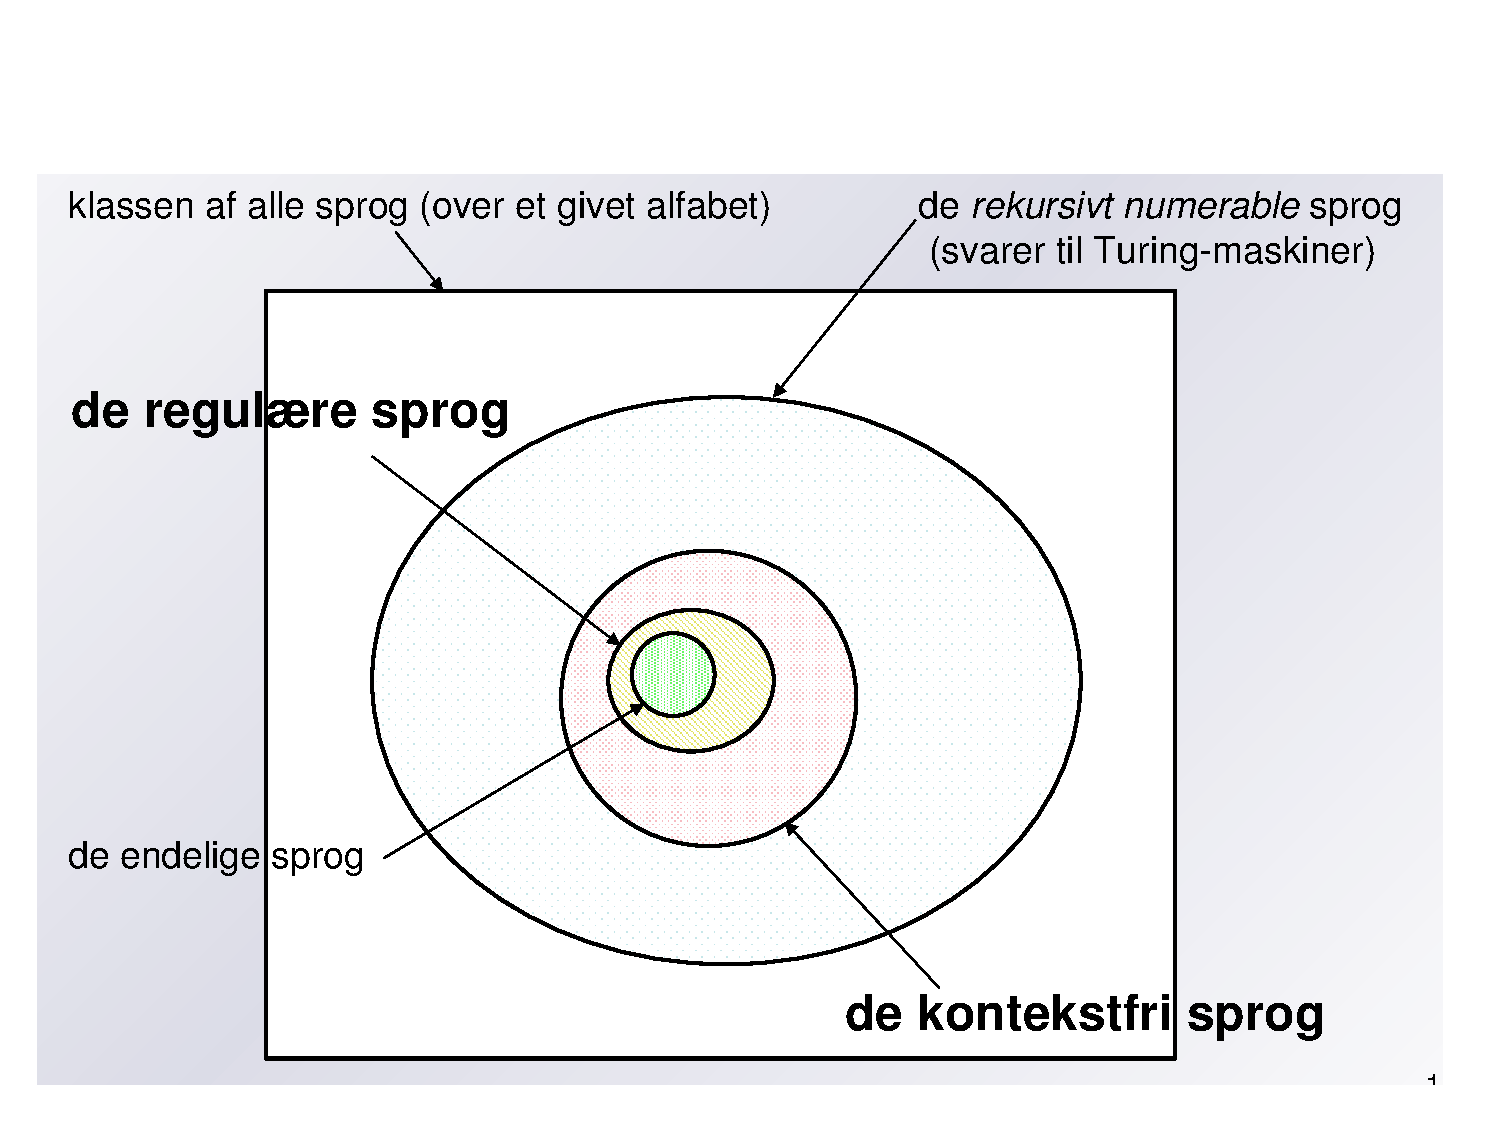
\includegraphics[scale=.4]{images/klasser}
\end{frame}

\begin{frame}
  \frametitle{Øvelser}
  \begin{itemize}[<+->]
  \item{} [Martin] 6.1 (a+b+e) (p. 240)
  \item{} [Martin] 6.9 (a-c) (p. 243)
  \end{itemize}
\end{frame}

\begin{frame}
\frametitle{Regulære sprog er også kontekstfri 1/2}
Der er simple konstruktioner for både $FA\rightarrow CFG$ og $regex \rightarrow CFG$
\begin{itemize}[<+->]
\item Givet en et regulært udtryk $r$ over alfabetet $\Sigma$ kan vi
konstruere en grammatik $G=(\{S\},\Sigma, S, P)$ så $L(G) = L(r)$
\item $r = \emptyset$ : $G=(\{S\},\Sigma, S, \emptyset)$
\item $r = \Lambda$ : $G=(\{S\},\Sigma, S, \{S\rightarrow \Lambda\})$
\item $r = a$ : $G=(\{S\},\Sigma, S, \{S\rightarrow a\})$
\end{itemize}
\end{frame}

\begin{frame}
\frametitle{Regulære sprog er også kontekstfri 2/2}
\begin{itemize}[<+->]
\item $r = r_1+r_2$ : $G=(\{S'\}\cup V_1 \cup V_2, \Sigma, S', \{S'\rightarrow S_1, S'\rightarrow S_2\} \cup P_1 \cup P_2)$

  Hvor $V_1, V_2$ er nonterminalerne i $G_1, G_2$, for de mindre regulære udtryk, men \alert{omdøbt så der ikke er konflikter}
\item $r = r_1\cdot r_2$ : $G=(\{S'\}\cup V_1 \cup V_2,\Sigma, S', \{S'\rightarrow S_1S_2\} \cup P_1 \cup P_2)$
\item $r = r_1^*$ : $G=(\{S'\}\cup V_1 \cup V_2,\Sigma, S', \{S'\rightarrow S_1, S'\rightarrow S'S_1, S' \rightarrow \Lambda\} \cup P_1 \cup P_2)$
\item Beviset for korrekthed er naturligvis induktion i strukturen af det regulære udtryk / strukturen af derivationen af $x\in G$.
\item Bemærk dette viser også at Kontekstfri sprog er lukket under $\cup$, konkatenering og ${}^*$

\end{itemize}
\end{frame}
\section{Afrunding, og om eksamen}
\begin{frame}
\frametitle{Eksamen}
\begin{itemize}
\item Der er 6 eksamensspørgsmål, man trækker et når man kommer ind.
\item Eksamen varer ca. 20 min inklusiv votering. Det er meget kort
  tid, så det er godt at have en konkret plan til hvert emne
\item Karakterer på den nye 7-trinsskala.
\item Brug endelig tavlen.
\end{itemize}
\end{frame}

\begin{frame}
  \frametitle{Eksamensspørgsmål} Her er forslag til hvilke emner man
  kunne komme ind på, bemærk dette er kun \emph{forslag}, og ikke bud
  på en færdig plan.\small{
  \begin{itemize}
  \item regulære udtryk (definition, skitse af Kleenes sætning, lav konstruktion $regex \rightarrow NFA-\Lambda$ og/eller $FA\rightarrow regex$)
  \item endelige automater (definition, produktkonstruktionen, dele af Kleene's sætning)
  \item lukkethedsegenskaber (produktkonstruktionen, homomorfier, regulære sprog lukket under ...)
  \item nondeterministiske automater (definition af NFA'er, determinisering, lambda-eliminering)
  \item minimering af automater (Uskelnelighed, MyHill Nerode, Minimeringsalgoritmen, $L_{42}$ har $2^{42}$ ækvivalensklasser)
  \item begrænsninger af regulære sprog (pumping-lemma, eksempler på ikke-regulære sprog, kontekstfrie grammatikker, klasser af sprog)
  \end{itemize}}
 \end{frame}
\end{document}
